\themaN
\graphicspath{{../Ch11_Tableaux_et_diagrammes/Images/}}

\chapter{Tableaux et\\graphiques}
\label{C26}


%%%%%%%%%%%%%%%%%%%%%%%%%%%%%%%%%%%%%%%%%
%%%%%%%%%%%%%%%%%%%%%%%%%%%%%%%%%%%%%%%%%
\begin{prerequis}[Connaissances et compétences associées]
   \begin{itemize}
      \item Prélever des données numériques à partir de supports variés. Produire des tableaux, diagrammes et graphiques organisant des données numériques.
      \item Exploiter et communiquer des résultats de mesures.
      \item Lire ou construire des représentations de données : tableaux (en deux ou plusieurs colonnes, à double entrée) ; diagrammes en bâtons ; graphiques cartésiens.
      \item Organiser des données issues d’autres enseignements (sciences et technologie, histoire et géographie, éducation physique et sportive, etc.) en vue de les traiter.
   \end{itemize}
\end{prerequis}

\vfill

\begin{debat}[Débat : le premier tableur]
   Des données brutes récoltées ont souvent peu de sens si elles sont utilisées ainsi, d'où la nécessité de les disposer d'une manière plus lisible à l'aide de tableaux et diagrammes. \\
   Avec l'avènement de l'informatique, les tableaux deviennent numériques grâce à l'apport des {\bf tableurs} : logiciels qui permettent de manipuler des données numériques, d'effectuer un certain nombre d'opérations de façon automatisée, de créer des représentations graphiques à partir des données : diagrammes , histogrammes, courbes\dots{} \\
   Le premier tableur fut créé en 1978 par {\it Daniel Bricklin}, étudiant à Harvard qui devait établir des tableaux comptables pour une étude de cas sur Pepsi-Cola sans pour autant établir tous les calculs \og à la main \fg. Son premier prototype, {\it VisiCalc} (pour Visible Calculator), pouvait manipuler un tableau de vingt lignes et cinq colonnes ! \\
   \begin{center}
      \textsf{
      \begin{tabular}{|>{\columncolor{lightgray!30}}c|*{5}{C{1}|}}
         \hline
         \rowcolor{lightgray!30} & A & B & C & D & E \\
         \hline
         1 & & & & &  \\
         \hline
         2 & & & & & \\
         \hline
         3 & & & & & \\
         \hline
     \end{tabular}}
   \end{center}
   \bigskip
   \begin{cadre}[B2][F4]
      \begin{center}
         Vidéo : \href{https://www.youtube.com/watch?v=mmyjICMR7BM}{\bf La petite histoire du tableur}, chaîne YouTube {\it Communauté dynamique}.
      \end{center}
   \end{cadre}
\end{debat}

\vfill

\textcolor{PartieGeometrie}{\sffamily\bfseries Cahier de compétences} : chapitre 6, exercices 1 à 26.


%%%%%%%%%%%%%%%%%%%%%%%%%%%%%%%%%%%%
%%%%%%%%%%%%%%%%%%%%%%%%%%%%%%%%%%%%
\activites

\begin{activite}[Récolter des données]
   {\bf Objectif :} récolter des données au sein de la classe afin de les représenter sous différentes formes. \\
   \begin{QCM}
      Quel est ton loisir préféré (sport, culture, art, jeu\dots) et combien de temps en minutes y consacres-tu en moyenne par semaine ?
      \begin{center}
      {\hautab{2.5}
      \begin{ttableau}{0.9\linewidth}{4}
         \hline
         & & & \\
         \hline
         & & & \\
         \hline
         & & & \\
         \hline
         & & & \\
         \hline
         & & & \\
         \hline
         & & & \\
         \hline
         & & & \\
         \hline
         & & & \\
         \hline
      \end{ttableau}}
      \end{center}
      \ \\
   \end{QCM}
\end{activite}


%%%%%%%%%%%%%%%%%%%%%%%%%%%%%%%%%%%%
%%%%%%%%%%%%%%%%%%%%%%%%%%%%%%%%%%%%
\cours 

%%%%%%%%%%%%%%%%%%%%%%%%%%%%%%%
\section{Tableaux}

On souhaite connaître les loisirs préférés ainsi que le temps passé en heures à pratiquer ce loisir d'une classe de 6\up{e} du collège Simone Veil composée ce jour-là de 25 élèves. On obtient les résultats suivants :
\begin{center}
   \begin{ttableau}{\linewidth}{5}
      \hline
      \colorbox{yellow}{Judo} \hfill 12 & \colorbox{red!50}{Rugby} \hfill 9 & \colorbox{gray!50}{Athlétisme} \hfill 3 & \colorbox{yellow}{Judo} \hfill 12 & \colorbox{cyan}{Jeux vidéo} \hfill 15 \\
      \hline
      \colorbox{red!50}{Rugby} \hfill 9 & \colorbox{lightgray}{Gymnastique} \hfill 6 & \colorbox{gray!50}{Vélo} \hfill 2 & \colorbox{yellow}{Judo} \hfill 16 & \colorbox{cyan}{Jeux vidéo} \hfill 20 \\
      \hline
      \colorbox{violet!50}{Dessin} \hfill 5 & \colorbox{cyan}{Jeux vidéo} \hfill 15 & \colorbox{yellow}{Judo} \hfill 10 & \colorbox{red!50}{Rugby} \hfill 9 & \colorbox{green}{Lecture} \hfill 4 \\
      \hline
      \colorbox{green}{Lecture} \hfill 4 & \colorbox{yellow}{Judo} \hfill 14 & \colorbox{gray!50}{Gymnastique} \hfill 4 & \colorbox{cyan}{Jeux vidéo} \hfill 12 & \colorbox{yellow}{Judo} \hfill 12 \\
      \hline
      \colorbox{yellow}{Judo} \hfill 14 & \colorbox{red!50}{Rugby} \hfill 15 & \colorbox{red!50}{Rugby} \hfill 9 & \colorbox{gray!50!}{Football} \hfill 10 & \colorbox{cyan}{Jeux vidéo} \hfill 13 \\
      \hline
   \end{ttableau}
\end{center}
 On organise les résultats : pour rassembler les données de manière pratique, on les présente sous forme d'un tableau à double entrée où l'on regroupe ensemble des activités de \og même type \fg. Par exemple :

\begin{exemple*1}
   \begin{center}  
   \renewcommand*\tabularxcolumn[1]{>{\centering\arraybackslash}m{#1}}
   \begin{Ctableau}{\linewidth}{7}{c}
      \hline
      Loisir & \colorbox{yellow}{\parbox{1.4cm}{Judo}} & \colorbox{red!50}{\parbox{1.4cm}{Rugby}} & \colorbox{lightgray}{\parbox{1.6cm}{Autres sports}} & \colorbox{cyan}{Jeux vidéo} & \colorbox{green}{Lecture} & \colorbox{violet!50}{Dessin} \\
      \hline
      Effectif & 7 & 5 & 5 & 5 & 2 & 1 \\
      \hline
      Durée en h. & 90 & 51 & 25 & 75 & 8 & 5 \\
      \hline
   \end{Ctableau}
   \end{center}
   \ \\ [-8mm]
\end{exemple*1}


%%%%%%%%%%%%%%%%%%%%%%%%%%%%%%%
\section{Diagrammes}

\begin{definition}
   Un \textbf{diagramme en bâtons} (ou en barres) est constitué de segments de droites verticaux dont chaque hauteur est proportionnelle au nombre qu'il représente. Il montre une répartition.
\end{definition}

\begin{exemple*1}
   Voici le diagramme en bâtons représentant les loisirs préférés de la classe de 6\up{e} : \\
   \begin{pspicture}(-3.3,-0.25)(12,6.8)
   {\psset{xunit=0.7,yunit=0.8}
   \footnotesize
      \psgrid[subgriddiv=0,gridlabels=0,gridcolor=lightgray!75](0,0)(-0.5,-0.5)(13,8)
      \psline{->}(0,0)(13,0)
      \multido{\i=1+1}{7}{\psline(-0.2,\i)(0.2,\i) \rput(-0.5,\i){\i}}
      \psline{->}(0,0)(0,8)
      \psset{linewidth=0.7,linecolor=A2}
      \psline(1.5,0)(1.5,7)
      \psline(3.5,0)(3.5,5)
      \psline(5.5,0)(5.5,5)
      \psline(7.5,0)(7.5,5)
      \psline(9.5,0)(9.5,2)
      \psline(11.5,0)(11.5,1)
      \rput(1.5,-0.5){Judo}
      \rput(3.5,-0.5){Rugby}
      \rput(5.5,-0.5){Autres}
      \rput(5.5,-1){Sports}
      \rput(7.5,-0.5){Jeux}
      \rput(7.5,-1){Vidéo}
      \rput(9.5,-0.5){Lecture}
      \rput(11.5,-0.5){Dessin}
      \rput(-1,7.7){\it Effectifs}
      \rput(14,0){\it loisirs}}
   \end{pspicture} 
\end{exemple*1}

\begin{remarque}
   les \og bâtons \fg{} ont une largeur quelconque, toujours la même sur la série.
\end{remarque}

\begin{definition}
   Un \textbf{diagramme circulaire} est constitué de secteurs circulaires dont la mesure des angles est proportionnelle aux effectifs. Il montre des proportions.
\end{definition}
   
\begin{exemple}
   Dans la classe de 6\up{e}, on a le diagramme circulaire suivant : \\
      {\psset{unit=0.8}
      \footnotesize
      \begin{pspicture}(-12,-3)(3,1.5)
         \pscircle(0,0){3}
         \pswedge(0,0){3}{0}{61}
         \pswedge[fillstyle=solid,fillcolor=A2](0,0){3}{0}{100.8}
         \pswedge[fillstyle=solid,fillcolor=A2!80](0,0){3}{100.8}{172.8}
         \pswedge[fillstyle=solid,fillcolor=A2!60](0,0){3}{172.8}{244.8}      
         \pswedge[fillstyle=solid,fillcolor=A2!40](0,0){3}{244.8}{316.8}
         \pswedge[fillstyle=solid,fillcolor=A2!20](0,0){3}{316.8}{345.6}
         \pswedge[fillstyle=solid,fillcolor=white](0,0){3}{345.6}{360}
         \rput(1.1,1.5){\white Judo}
         \rput(1.1,1.1){\white 28\,\%}
         \rput(-1.5,1.3){\white Rugby}
         \rput(-1.5,0.9){\white 20\,\%}
         \rput(-1.6,-0.7){\white Autres sports}
         \rput(-1.4,-1.1){\white 20\,\%}
         \rput(0.3,-1.6){Jeux vidéo}
         \rput(0.3,-2){20\,\%}
         \rput(1.9,-0.8){Lecture}
         \rput(2.1,-1.2){8\,\%}
         \rput(2.1,-0.2){Dessin 4\,\%}
      \end{pspicture}}  
\end{exemple}


%%%%%%%%%%%%%%%%%%%%%%%%%%%%%%%%%%%%%%
\section{Graphique cartésien}

\begin{definition}
   Un \textbf{graphique cartésien} est une représentation qui permet de visualiser l'évolution d'une grandeur (en ordonnées) \og en fonction \fg{} d'une autre (en abscisse).
\end{definition}

\smallskip

\begin{exemple*1}
   Le tableau suivant donne les températures minimales et maximales moyennes mensuelles à Montpellier sur la période 1981-2010. \\ [3mm]
   {\small
   \hautab{1.5}
   \begin{Ltableau}{\linewidth}{13}{c}
      \hline
      Mois & janv & fév & mars & avril & mai & juin & juil & août & sept & oct & nov & déc \\
      \hline
      Temp. minimale en C\degre & 2,8 & 3,3 & 5,9 & 8,7 & 12,5 & 16,0 & 18,9 & 18,5 & 15,0 & 11,9 & 6,8 & 3,7 \\
      \hline
      Temp. maximale en C\degre & 11,6 & 12,8 & 15,9 & 18,2 & 22,0 & 26,4 & 29,3 & 28,9 & 25,0 & 20,5 & 15,3 & 12,2 \\
      \hline
   \end{Ltableau}
   \psset{yunit=0.2,xunit=0.88}
   \begin{pspicture}(-1.5,-1)(13,35)
      \psaxes[Dy=5]{->}(0,0)(13.5,32)
      \psdots[dotstyle=+,dotscale=1.5,linecolor=A1](1,2.8)(2,3.3)(3,5.9)(4,8.7)(5,12.5)(6,16)(7,18.9)(8,18.5)(9,15)(10,11.9)(11,6.8)(12,3.7)
      \psline[linecolor=A1,linewidth=0.03](1,2.8)(2,3.3)(3,5.9)(4,8.7)(5,12.5)(6,16)(7,18.9)(8,18.5)(9,15)(10,11.9)(11,6.8)(12,3.7)
      \psdots[dotstyle=+,dotscale=1.5,linecolor=B1](1,11.6)(2,12.8)(3,15.9)(4,18.2)(5,22)(6,26.4)(7,29.3)(8,28.9)(9,25)(10,20.5)(11,15.3)(12,12.2)
      \psline[linecolor=B1,linewidth=0.03](1,11.6)(2,12.8)(3,15.9)(4,18.2)(5,22)(6,26.4)(7,29.3)(8,28.9)(9,25)(10,20.5)(11,15.3)(12,12.2)
      \rput(0,33){\it Température en C\degre}
      \rput(14.3,0.7){\it Numéro}
      \rput(14.3,-0.7){\it du mois}
   \end{pspicture}}  
\end{exemple*1}

\medskip

%%%%%%%%%%%%%%%%%%%%%%%%%%%%%%%%%%%
%%%%%%%%%%%%%%%%%%%%%%%%%%%%%%%%%%%
\exercicesbase

\begin{colonne*exercice}

\serie{Lire et interpréter des données}

\begin{exercice} %1
   Voici un extrait d'horaires de la ligne 10 du bus du réseau TAM de Montpellier et de son agglomération en direction de Celleneuve le dimanche.
   \begin{center}
      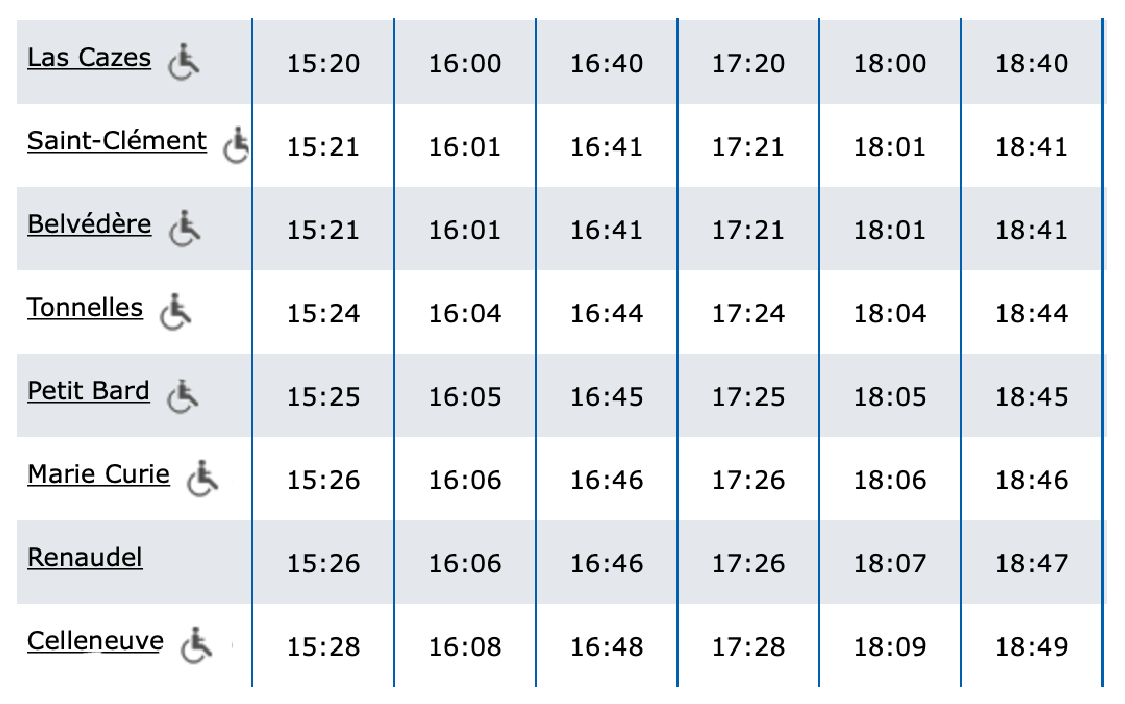
\includegraphics[width=8.1cm]{ligne10} \\ [-2mm]
      \hfill {\footnotesize\it Source : TAM, 2019}
   \end{center}
   \begin{enumerate}
      \item Que signifie le pictogramme présent à côté de certaines stations ?
      \item Fatima a donné RDV à ses copines devant le collège à 16h25 afin de prendre le bus à l'arrêt Las Cazes pour aller à Renaudel. À quelle heure prendront-elles le bus et à quelle heure arriveront-elles ?
      \item Jules part de Saint-Clément et va jusqu'à Marie-Curie, il doit y être avant 18h. Quel bus doit-il prendre ?
      \item Combien de temps faut-il pour aller de Las Cazes à Petit Bard ?
   \end{enumerate}
\end{exercice}

\begin{exercice} %2
   Le diagramme ci-dessous représente les meilleures ventes de jeux vidéo toutes plates-formes confondues en France en 2018, en milliers d'unités.
   \begin{center}
      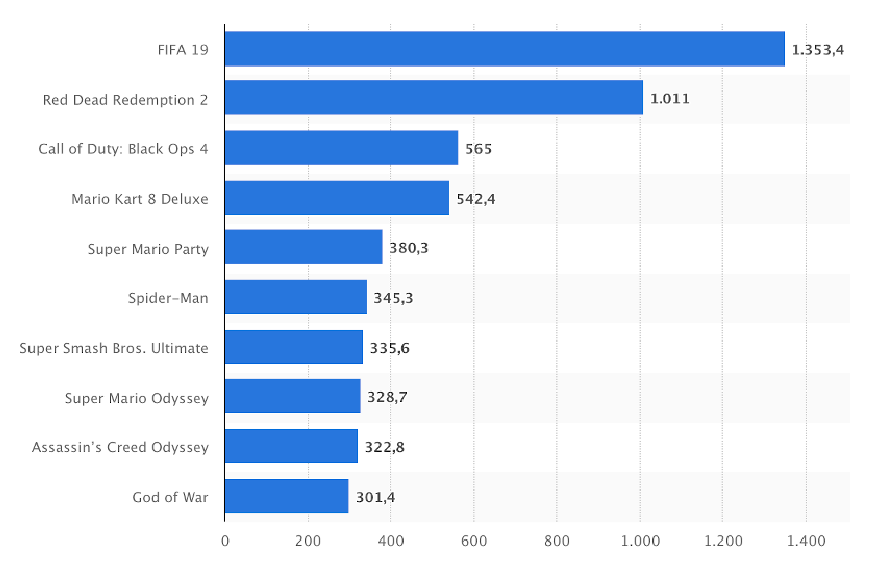
\includegraphics[width=8cm,height=6cm]{jeux_video} \\ [-2mm]
      \hfill {\scriptsize\it Source : Statistica.com, 2019}
   \end{center}
   \begin{enumerate}
      \item Quel a été le jeu le plus vendu en 2018 ?
      \item Combien de jeux ont été vendus à plus de 350 000 unités ?
      \item Au total, combien de jeux \og Mario \fg{} ont été vendus ?
   \end{enumerate}
\end{exercice}

\begin{exercice} %3
   Le diagramme ci-dessous représente la répartition des hommes et des femmes suivant leur indice de masse corporelle (I.M.C.).
   \begin{center}
      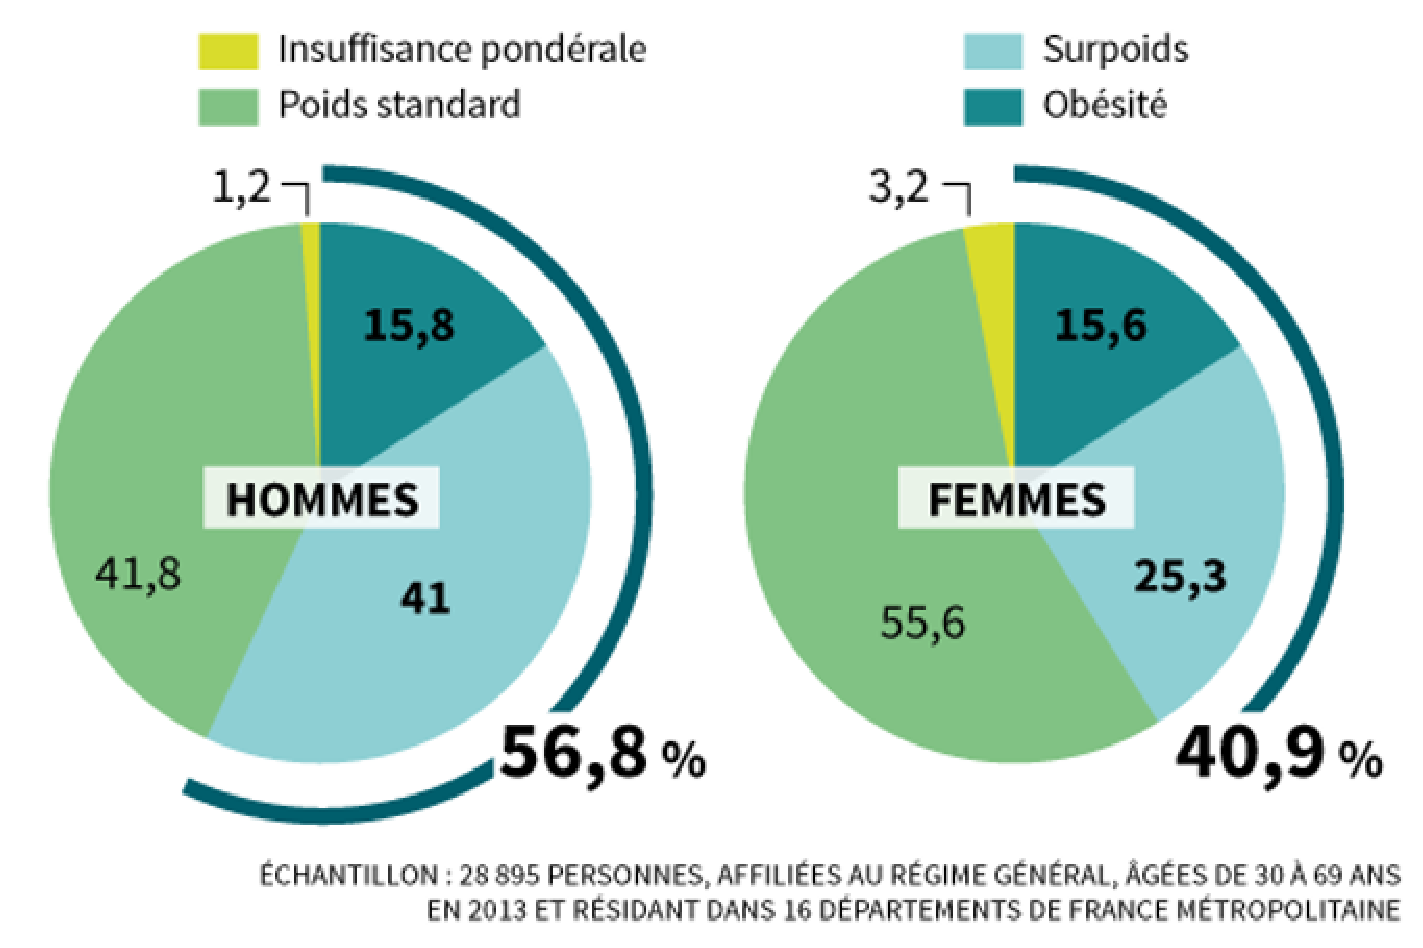
\includegraphics[width=7cm]{surpoids} \\ [-2mm]
      \hfill {\scriptsize\it Source : Santé publique française, Bulletin épidémiologique, 2016}
   \end{center}
   \begin{enumerate}
      \item Qu'est-ce que l'I.M.C. ?
      \item En moyenne, qui des hommes ou des femmes sont le plus affectés par le surpoids ?
      \item Quel est le pourcentage de femmes en obésité ?
      \item Quel est le pourcentage d'hommes en insuffisance pondérale ?
      \item Quelle est la catégorie la plus représentée chez les hommes ?
   \end{enumerate}
\end{exercice}

\begin{exercice} %4
   La Mascareignes est un ultra-trail se déroulant sur l'île de la Réunion.
   \begin{center}
      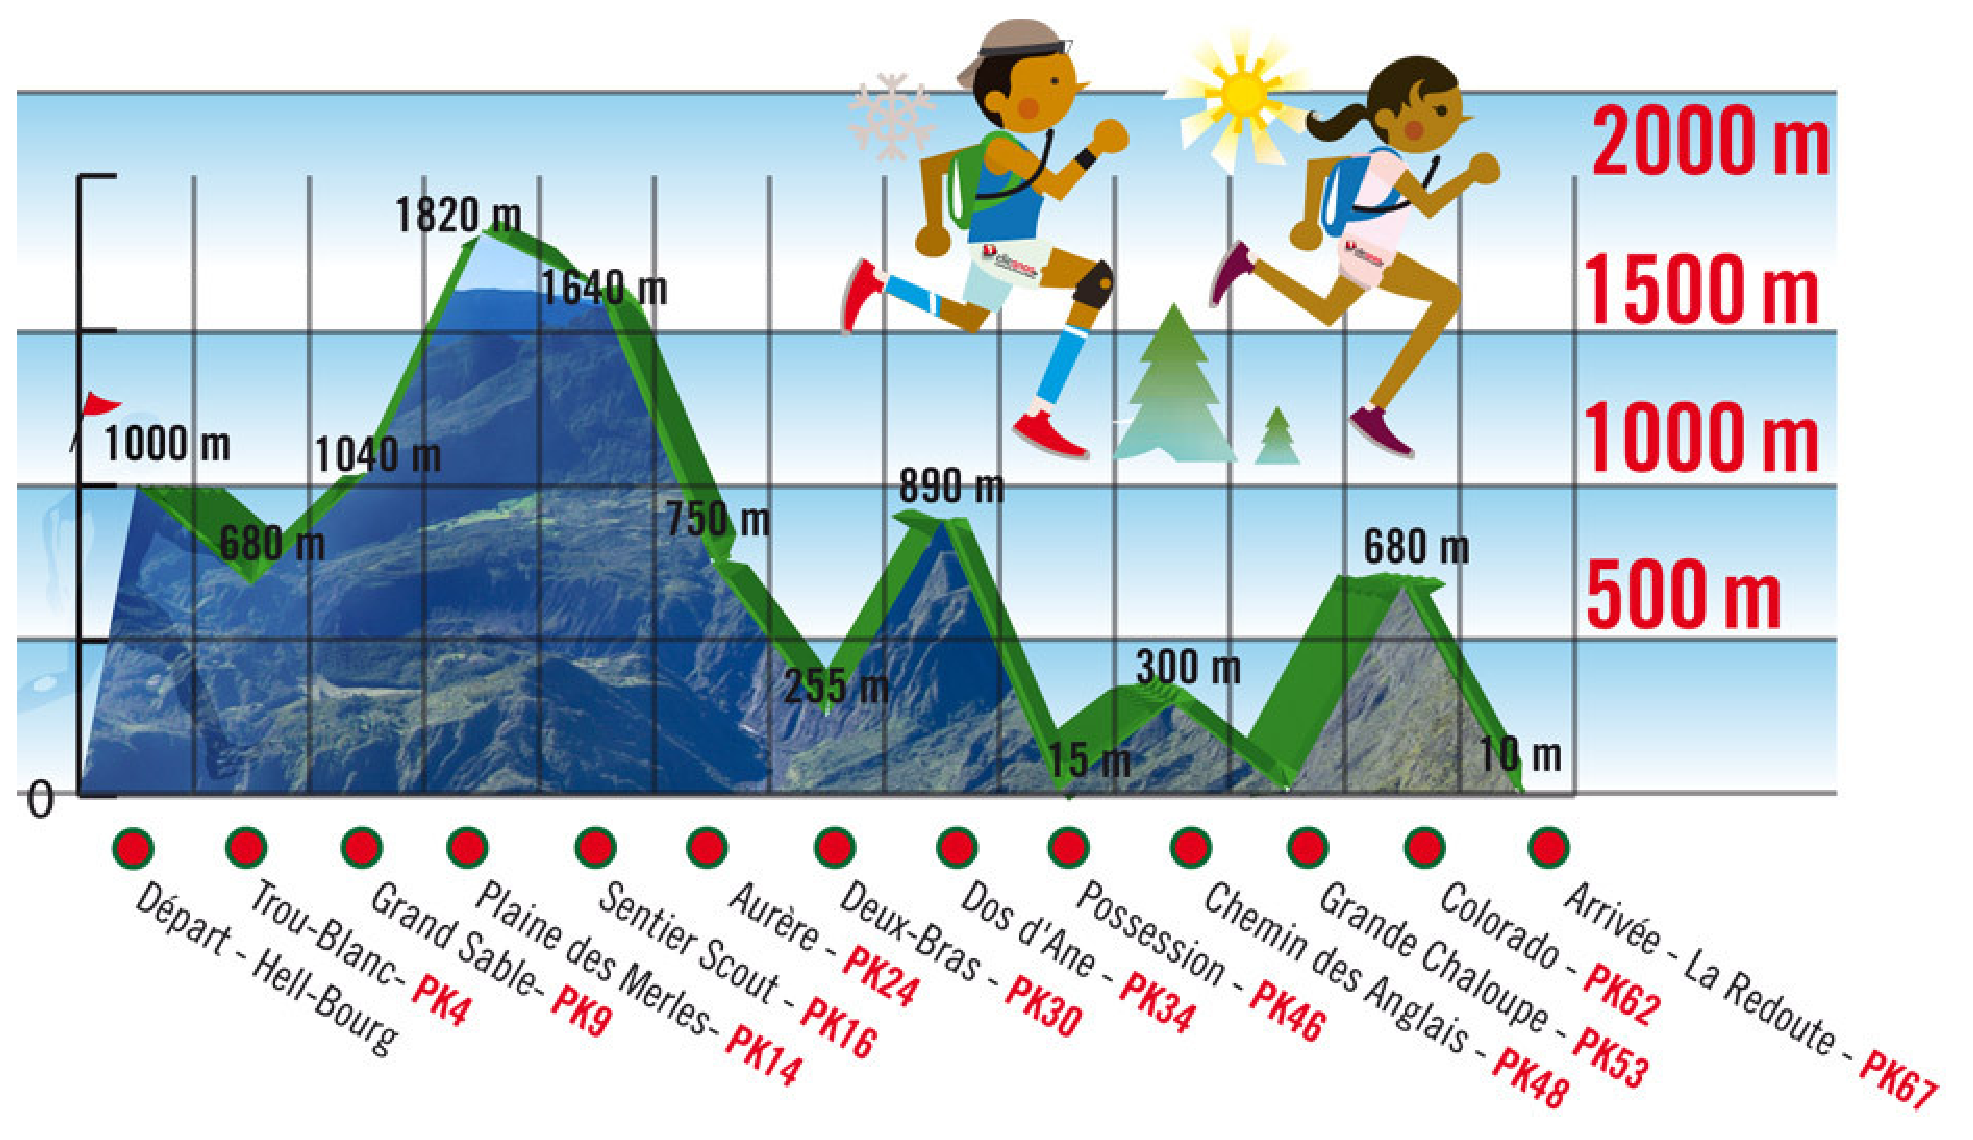
\includegraphics[width=8.5cm,height=5.5cm]{Mascareigne} \\ 
      \hfill {\footnotesize\it Source : La Réunion lé la, overblog, 2016}
   \end{center}
   D'après le diagramme cartésien ci-dessus représentant le dénivelé en fonction du lieu, répondre aux questions suivantes :
   \begin{enumerate}
      \item Que signifie \og PK14 \fg ?
      \item Quelle est la longueur de la course ?
      \item Où se situe l'altitude la plus élevée ? Quelle est cette altitude ?
      \item Combien y-a-t-il de km entre Grand-Sable et la Grande Chaloupe ?
      \item Quel est le dénivelé entre le début du Sentier Scout et Deux-bras ?
      \item À peu près combien de km parcourt-on au delà de 1\,000 m d'altitude ?
   \end{enumerate}
\end{exercice}

\bigskip

\serie{Représenter des données} %%%%%%%%

\begin{exercice} %5
   L'infographie suivante donne le nombre de fois que des sortilèges de magie apparaissent dans les sept livres de la série {\it Harry Potter}.
   \begin{center}
      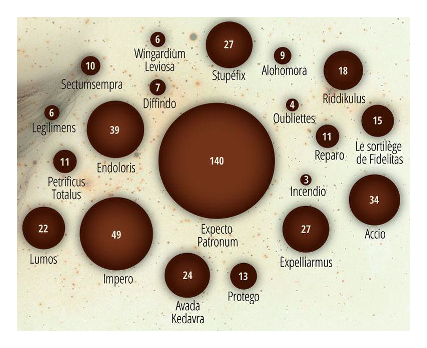
\includegraphics[width=8cm]{infographie_HP} \\
      \hfill {\footnotesize\it Source : Harry Potter, les nombres d'or de la saga, Le Figaro.fr, 2017}
   \end{center}
   \begin{enumerate}
      \item Comment sont représentées les données dans cette infographie ?
      \item Combien y a-t-il eu de sortilèges donnés au total dans les sept livres ?
      \item Représenter les données dans un tableau en notant uniquement les sortilèges cités plus de 20 fois.
      \item Construire un diagramme en bâtons pour les valeurs de ce tableau. \\
   \end{enumerate}
\end{exercice}

\begin{exercice} %6
   Le tableau ci-dessous représente la répartition des médailles françaises aux Jeux olympiques (JO) d'été de 1896 à 2016 pour les dix sports ayant eu le plus de médailles.
   \begin{enumerate}
      \item Compléter le tableau.
      \item Comment est établi le classement des sports aux JO ?
   \end{enumerate}
   \begin{center}
      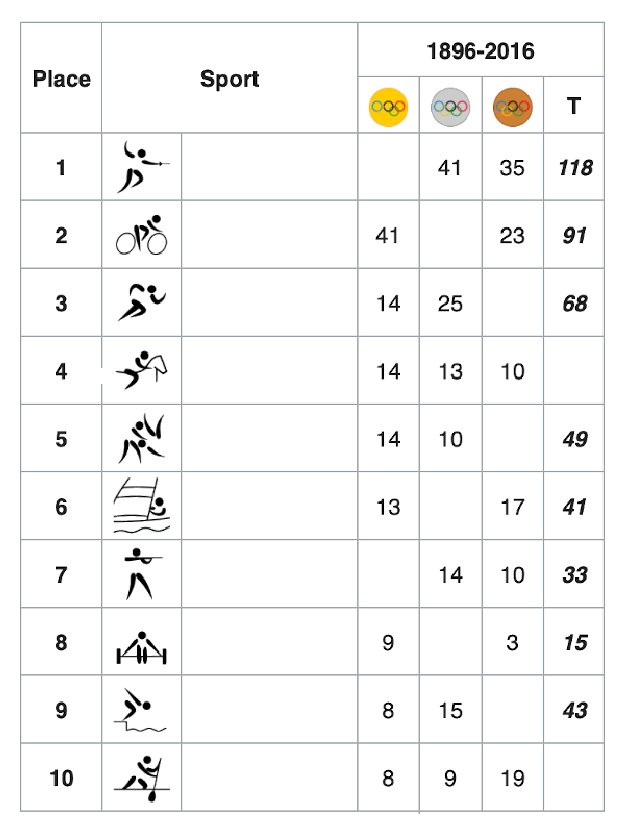
\includegraphics[width=8cm]{JO_trous} \\
      \hfill {\footnotesize\it Source : France aux Jeux olympiques, Wikipedia, 2019}
   \end{center}
\end{exercice}

\begin{exercice}
   Le tableau suivant donne l'évolution de la population de Montpellier depuis un siècle.
   \begin{center}
   {\small
   \hautab{1.6}
      \begin{tabular}{|p{1.5cm}|*{5}{C{0.9}|}}
      \hline
      Année & 1921 & 1931 & 1946 & 1962 & 1975 \\
      \hline
      Population & 81\,548 & 86\,924 & 93\,102 & 118\;864 & 191\,354 \\
      \hline
      Année & 1982 & 1999 & 2006 & 2011 & 2016 \\
      \hline
      Population & 197\,231 & 225\,392 & 251\,634 & 264\,538 & 281\,613 \\
      \hline
   \end{tabular} \\ [2mm]
   \hfill {\scriptsize\it Source : Montpellier, Wikipedia, 2019}}
   \end{center}
   \begin{enumerate}
      \item Construire un diagramme cartésien représentant ce tableau. On prendra \ucm{1} pour 5 années en abscisses et \ucm{1} pour 20\,000 habitants en ordonnées.
      \item Que peut-on dire de cette évolution ?
   \end{enumerate}
\end{exercice}

\end{colonne*exercice}


%%%%%%%%%%%%%%%%%%%%%
%%%%%%%%%%%%%%%%%%%%%
\Recreation

\enigme[Tâche complexe : sorties au cinéma.]
Misgana a 12 ans. Elle veut organiser des sorties au cinéma avec trois de ses camarades du même âge qu'elle, pendant la première semaine des vacances scolaires de la Toussaint. Les vacances commencent le samedi 19 octobre et se terminent le dimanche 3 novembre. \\
Misgana demande à ses camarades quels sont les jours et les heures qui leur conviennent pour cette sortie. Elle a reçu les informations suivantes :
\begin{itemize}
   \item Ciana : \og Je dois rester chez moi le lundi et le mercredi après-midi de 14h30 à 15h30 pour mes leçons de danse \fg.
   \item Sofia : \og Je dois revenir pour 17 h car j'ai besoin de lire au moins 2 h avant le dîner \fg.
   \item Q'Orianka : \og J'ai des compétitions de natation synchronisée les dimanches, donc les dimanches sont exclus. J'ai déjà vu Pokamin et je ne veux pas le revoir \fg.
\end{itemize}
Misgana doit choisir des films qui ne sont pas interdits aux jeunes de son âge et ses parents insistent pour qu'elle ne rentre pas à pied ; ils proposent de ramener les filles chez elles à n'importe quelle heure jusqu'à 22 h. Elle se renseigne sur les programmes de cinéma pour la première semaine de vacances. Voici les informations qu'elle a recueillies :
\begin{center}
   {\small
   \begin{tabular}{|p{4cm}p{1.8cm}|p{4cm}p{1.8cm}|}
      \hline
      \multicolumn{4}{|c|}{\bf Cinéma Setièmard} \\
      \multicolumn{4}{|c|}{Réservations au numéro : 08 00 42 30 00} \\
      \multicolumn{4}{|c|}{Programme en vigueur à partir du mercredi 16 octobre pour deux semaines.} \\
      \hline
      \bf Hari Kover & & \bf Pokamin & \\
      113 min & Interdit aux & 105 min & Accord \\
      14h00 (lun.-ven. seulement) & moins de & 13h40 (tous les jours) & parental \\
      21h35 (sam.-dim. seulement) & 12 ans. & 16h35 (tous les jours) & souhaitable. \\
      \hline
      \bf Le monstre des profondeurs & & \bf Enigma & \\
      164 min & Interdit aux & 144 min & Interdit aux \\
      19h55 (ven.-sam. seulement) & moins de & 15h00 (lun.-ven. seulement) & moins de \\
      & 18 ans. & 18h00 (sam.-dim. seulement) & 12 ans. \\
      \hline
      \bf Carnivore & & \bf Le roi de la savane & \\
      148 min & Interdit aux & 117 min & Pour tous. \\
      18h30 (tous les jours) & moins de & 14h35 (lun.-ven. seulement) & \\
      & 18 ans. & 18h50 (sam.-dim. seulement) & \\
      \hline
   \end{tabular}}
\end{center}

Quel planning Misgana va-t-elle proposer à ses amies afin de voir un maximum de films ? Pour aider à organiser les résultats, on pourra utiliser un tableau de ce type :
\begin{center}
   \small
   \begin{tabular}{|p{1.5cm}|p{1.5cm}|p{1.5cm}|p{1.5cm}|p{1.5cm}|p{1.5cm}|p{1.5cm}|p{1.5cm}|}
      \hline
      horaire & samedi & dimanche & lundi & mardi & mercredi & jeudi & vendredi \\
      & 19 octobre & 20 octobre & 21 octobre & 22 octobre & 23 octobre & 24 octobre & 25 octobre \\
      \hline
      13h & & & & & & & \\ [1.5mm]
      14h & & & & & & & \\ [1.5mm]
      15h & & & & & & & \\ [1.5mm]
      16h & & & & & & & \\ [1.5mm]
      17h & & & & & & & \\ [1.5mm]
      18h & & & & & & & \\ [1.5mm]
      19h & & & & & & & \\ [1.5mm]
      20h & & & & & & & \\ [1.5mm]
      21h & & & & & & & \\ [1.5mm]
      22h & & & & & & & \\ [1.5mm]
      23h & & & & & & & \\ [1.5mm]
      \hline
   \end{tabular}
\end{center}

\hfill {\footnotesize\it Source : adapté de PISA 2003 et Tâches complexes cycle 4, \url{https://pedagogie.ac-reims.fr} }

